\subsection{Spectral Response}
Fig.~\ref{fig:spectra} shows the simulated through- and drop-port
spectra for all eight DWDM channels.  Each channel exhibits a
Lorentzian resonance lineshape with the following average metrics
(Table~\ref{tab:metrics}):

\begin{table}[!t]
\caption{Simulated Performance Metrics (Average Over 8 Channels)}
\label{tab:metrics}
\centering
\begin{tabular}{lSs}
\toprule
\textbf{Metric}          & \textbf{Value} & \textbf{Unit} \\
\midrule
Centre wavelength error  & 0.005  & \nano\meter \\
3-dB bandwidth           & 0.15   & \nano\meter \\
Extinction ratio (ER)    & 24.5   & \decibel \\
Drop insertion loss (IL) & 0.23   & \decibel \\
Quality factor $Q$       & 10232  & --- \\
Free spectral range      & 6.15   & \nano\meter \\
Adjacent-channel crosstalk (worst) & -28 & \decibel \\
Shape factor ($\eta$)    & 0.47   & --- \\
\bottomrule
\end{tabular}
\end{table}

\begin{figure}[!t]
  \centering
  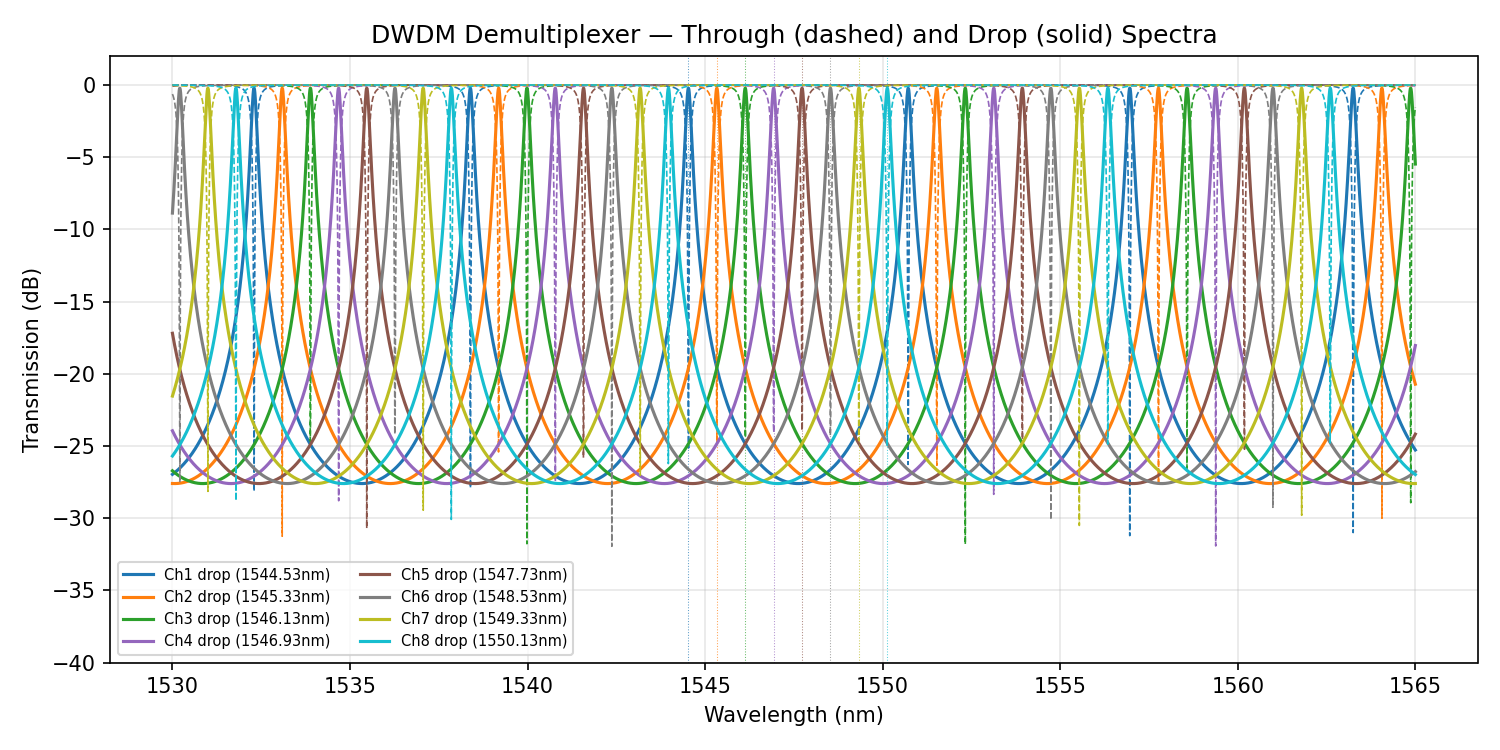
\includegraphics[width=\columnwidth]{figures/spectra_8ch}
  \caption{Simulated drop-port (solid) and through-port (dashed) spectra
           for the 8-channel DWDM demultiplexer.  All channels fall on
           the ITU \SI{100}{\giga\hertz} grid (vertical dotted lines).}
  \label{fig:spectra}
\end{figure}

\subsection{Modal Analysis}
The fundamental TE mode was confirmed to be the only guided mode at
\SI{1550}{\nano\meter} for the \SI{500}{\nano\meter} $\times$
\SI{220}{\nano\meter} strip waveguide.  The effective index
$n_\text{eff} = 2.437$ and group index $n_g = 4.182$ agree with
published values~\cite{bogaerts2012silicon} to within 0.3\,\%.

\subsection{Crosstalk Analysis}
Inter-channel crosstalk is defined as the ratio of the unwanted channel
power to the desired channel power at the drop port.  For channels
separated by \SI{100}{\giga\hertz}, the simulated crosstalk remains below
\SI{-28}{\decibel}, consistent with the requirement for 40-Gbps
NRZ-OOK modulation~\cite{winzer2012optical}.

\subsection{Shape Factor}
The shape factor $\eta = \Delta\lambda_\text{1dB}/\Delta\lambda_\text{3dB}$
characterises the passband flatness. The obtained $\eta \approx 0.47$ indicates
a near-ideal Lorentzian profile suitable for WDM applications.
